\section{Process' Perspective}
\label{ch:background} 

\subsection{CI/CD pipeline using GitHub actions}
%A complete description of stages and tools included in the CI/CD chains, including deployment and release of your systems.
Our CI/CD pipeline is shown in Figure \ref{fig:activity_diagram}, which illustrates the process 
of creating a ticket about a feature or an issue,
developing the feature or fixing the issue, creaating a pull request (PR),
reviewing the PR, merging it into the main branch, and finally realeasing and deploying the application.
\begin{figure}[h]
      \centering
      \makebox[\linewidth]{
      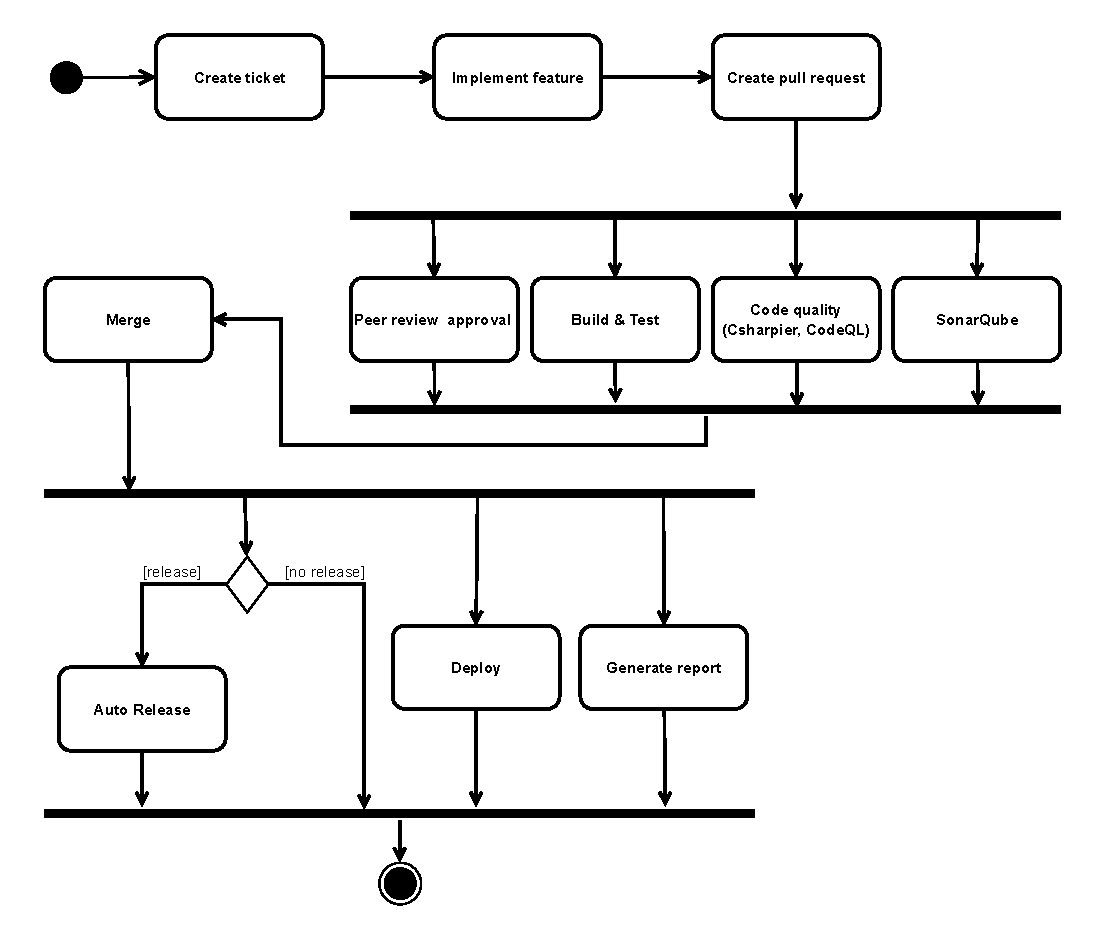
\includegraphics[width=1.4\textwidth]{images/activity_diagram.drawio.pdf}}
      \caption{Activity diagram of the CI/CD pipeline}
      \label{fig:activity_diagram}
\end{figure}

We use GitHub issues to create tickets for new features and issues.
The CI/CD pipeline is implmented using GitHub actions to automate the
building, testing, analysis of code quality, releasing, and deployment
of the MiniTwit application.
The pipeline consists of multiple workflows: build-test.yml, codeql.yml, auto-merge-dependabot.yml, auto-release.yml, and deploy.yml. 
Workflows are located at \textit{.github/workflows} in the repository. 

\subsubsection{Build and Test Workflow}
This workflow is triggered on every PR to \textit{main}.
The purpose of this is to build the application, run unit tests, 
and generate/upload a code coverage report.
Passing this workflow is a requirement for merging PR's into \textit{main}.

\subsubsection{Code Quality Workflow}
This workflow makes use of GitHub's \texttt{CodeQL} to perform static code analysis 
of C\# code only.
This workflow uses the same triggers as the build and test workflow, however, 
it is also triggered on a schedule, which is set to run every Thuesday via CRON.
Before performing the analysis, it formats the C\# code using \texttt{csharpier} to 
ensure consistency and automatically commits and pushes formatting changes.
It then performs a sematics code analysis to find security vulnerabilities and 
automatically uploads the results to GitHub, which is displayed on PR's.
This became very relavant when it once discovered that we leaked a third party 
API key in our code, which we then removed and updated.

Addtionally, we use SonarQube, CodeFactor, and OpenSSF to perform code analysis 
such as code coverage, duplication, security risks, and other best practices.
SonarQube's analysis is done by using \texttt{sonarcloud-github-action}, which 
uploads the results to SonarCloud, and is displayed on the PR.
CodeFactor and OpenSSF have read access to our repository, and automatically 
perform code analysis whenever our repository is updated.
The updated results are displayed on the front page of the repository on GitHub as batches.

\subsubsection{Auto Merge Dependabot Workflow}
Our project uses \texttt{dependabot} to automatically update dependencies in the project.
We have a GitHub action that detects PR's created by dependabot, and automaticaly merges 
them into \textit{main} if all workflows pass.
This was done to ensure that we always have the latest dependencies,
and to avoid having to manually merge dependabot PR's.

\subsubsection{Auto Release Workflow}
This workflow was inspired by a GitHub actions auto release template\cite{auto-release}.
It is triggered on every push to the \textit{main} branch, and automatically 
creates a new release on GitHub.
It requires a commit containing a message in the format \texttt{Release: x.y}, 
where x and y are the major and minor version numbers, respectively.
To add title and release note information, this is added to the file \textit{CHANGELOG.md}.
The purpose of this is to automate the release process, to replace the process 
of manually create a release on GitHub every time we want to release a new version 
of the application.

\subsubsection{Deployment Workflow}
This workflow is triggered on succesful completion of the build and test workflow 
after push to main.
It is responsible for building docker images, uploading, and deploying them to 
Digital Ocean droplets.
To deploy, it uses Docker Hub to authenticate and push the built images.
It uses \texttt{scp} and \texttt{ssh} to copy two remote files \texttt{deploy.sh} 
and \texttt{docker-compose.yml} to the relevant droplet,
which are then executed to deploy the application.
For deployment safeguards; SSH keys, IP addresses, and creditials are stored in GitHub secrets,
which are then used in the workflows to access the Digital Ocean droplets and to 
authenticate with Docker Hub.


\subsection{Terraform}
Terraform is used to provision and manage our infrastructure as code, 
to automatically setup droplets in Digital Ocean. 
The result of the Terraform setup is illustrated 
in Figure \ref{fig:deployment_diagram}.
Terraform creates all droplets with SSH keys and files.
It also configures the docker swarm for the API.
It then calls the deploy scripts on each droplet.
Finally it asssignes the reserved IP's.

To maintain infrastructure consistency and avoid creating duplicate droplets,
the Terraform state file is shared in a remote Digital Ocean Spaces.

\subsection{Logging and monitoring}
Serilog is used for logging API requests, responses, and errors.
Together with Seq, we can view the logs in a web interface to monitor 
applciation activity, and display graphs containing application performance 
for developers, and business statistics for stakeholders to use.
In Seq, we have three dashboards: overview, endpoint overview, and business.
The overview dashboard contains a general view of the application 
errors/exceptions, and the total number of events.
The endpoint overview dashboard contains a view of the API endpoints,
showing the number of requests, and average response times.
Lastly, the business dashboard contains a view of user activity,
showing when and how often users posts tweets, and the total number of tweets over time.


\subsection{Security assessment}
To analyse security risks in our code, we use tools like GitHub's CodeQL\cite{codeql} that 
integrated with our CI/CD pipeline.
This provides a display of security vulnerabilities in our code,
which is shown on the PR's.

To analyse security risks of the droplets, Docker Scout have been used to get
quick overviews of security risks from our docker images.
It scores the images in four levels: low, medium, high, and critical.
Addtionally, it provides recommendations on how to fix the issues.


Additionally, we use a risk assessment matrix to assess the probability and impact of security risks. 
These are split of into; probability (unlikely, possible, likely) and impact (negligible, moderate, and catastrophic).
\begin{itemize}
      \item \textif{Access to Seq monitoring tool (negligible, likely)}: In the case of resetting/failure of the Seq droplet, the logs are lost. Morever, the Seq password is reset everytime, as we do not have any fail safe default. Giving malicious users temporary access to our Seq dashboards, until we reset the password. However, this is not a big issue, as Seq is only used for monitoring and logging, and does not contain any sensitive information. However, only one user (stakeholder or developer) can access Seq at a time, which can be abused to deny availability to legitimate users.
      \item \textif{Login credentials leaked (moderate, likely)}: Usernames and passwords are stored in plaintext in our database (no encrpytion or hashing applied). If an attack agains read access to the users table, all credentials are immediately comprised. Leading to unathorized account takeover. 
      \item \textif{Overloading the API with requests (moderate, possible)}: A DDoS (distributed denial of service) attack can flood our API with axcessive traffic, rendering it unavailable to legitimate users. Basic load-balancing and firewall configuration exists, but there is no safe guard against DDoS attacks. Neither do we enfornce CAPTCHA or rate-limiting on critical endpoints. The impact is limited to service unavailablity. 
      \item \textif{Access to the database (catastrophic, unlikely)}: If an attack obtains direct database credentials or exploits a vulnerability to gain read/write access. They could delete or modify critical data, or have access to all user data, including usernames and passwords.
      \item \textif{Leak of secrets and API keys (catastrophic, possible)}: Secrets are sometimes shared informally (e.g., via Discord). Thus if the wrong person is invited, these keys could be exposed. An attacker with a valid API key could impersonate our services, or cause damage. The probability is possible until stricter secret-amangement policies are enforced, such as using a secret manager or vault.
      \item \textif{Failure of the Digital Ocean droplets (catastrophic, possible)}: Any droplet could fail due to software or hardwaere issues. We currently have no automated database backups; if the database droplet dies, we lose all data. TThe impact is catastrophic as we could lose all data (including user accounts and tweets) and the application would be unavailable until the droplet is restored or replaced.
\end{itemize}

\subsection{Scaling}

Client is scalable since it is client side rendered.
Api is scalable as it is stateless and uses docker swarm.

\subsection{AI-assistants}

Gpt was of great help in translating python to csharp.
Generating files.
Not so great at ...?